\subsection{bash}
\emph{bash} (Bourne-again shell) är en kommandotolk som är vanligt på unix-liknande system som Ubuntu och OSX. 
\paragraph{Funktionalitet}
En stark funktionalitet hos \emph{bash} är dess kraftfulla förmåga att använda shellglobar för att matcha filnamn.
Shellglobbing är motsvarigheten av reguljära uttryck för filer och kataloger. Karaktären * används för att matcha alla karaktärer i en sträng.
\newpage
\paragraph{Exempel: matchning av filtyper}
\begin{center}
        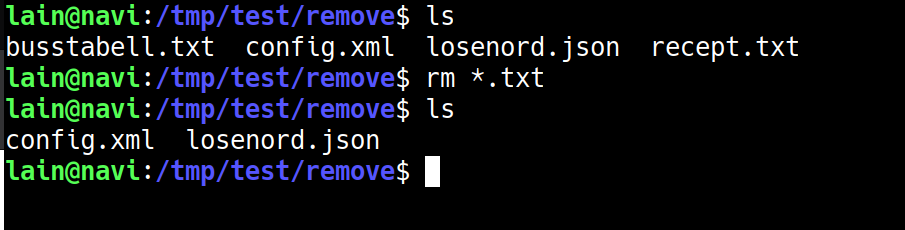
\includegraphics[width=\linewidth]{bilder/bash_remove_filetype.png}
        \captionof{figure}{Filer raderas efter filtyper}
\end{center}
I exemplet används * för att matcha alla filnamn som slutar med .txt och därefter effektivt raderar kommandot alla textfiler.
\paragraph{Exempel: matchning av alla filer}
\begin{center}
        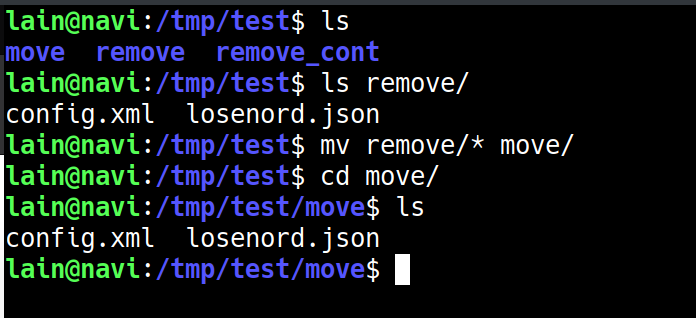
\includegraphics[width=\linewidth]{bilder/bash_move_files.png}
        \captionof{figure}{Filer flyttas från en katalog till en annan katalog}
\end{center}
Kommandot i figuren matchar alla filer i en katalog och flyttar över dem till en annan katalog.
\paragraph{Exempel: matchning av innehåll i filnamn}
\begin{center}
        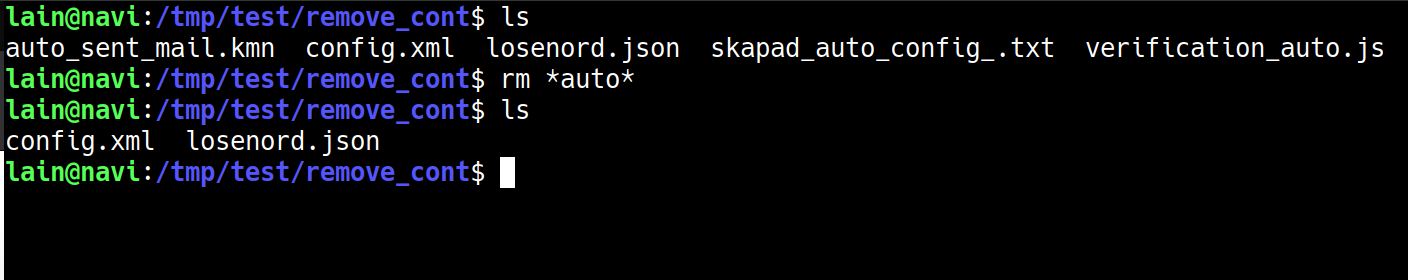
\includegraphics[width=\linewidth]{bilder/bash_remove_files_cont.png}
        \captionof{figure}{Filer raderas efter innehåll i deras filnamn}
\end{center}
I figuren visas hur man i bash kan använda globbing för att matcha filer som innehåller ett visst nyckelord och ta bort dem.
